\chapter{Experimentos Computacionais}
\label{chap:experiments}

\noindent Com o problema delineado, um modelo matemático pronto (TATSP) e três abordagens distintas implementadas, seguimos para a seção de experimentos visando avaliar o desempenho de cada ideia proposta.

Para realizar os experimentos foi utilizado um ambiente Ubuntu $22.04$, com $16$GB de RAM e um processador Intel Core $i7-12700H$ de $2.30$ GHz. Além disso o \emph{solver} escolhido foi o \emph{Gurobi} sob uma licença acadêmica e a linguagem de programação utilizada para implementar as abordagens foi Julia na versão $1.11$.

Os experimentos realizados se utilizam de instâncias fornecidas na competição MESS2024~\cite{MESS2024}. Dada a extensa lista de instâncias, foram selecionadas três instâncias de cada grupo, totalizando 6 instâncias, sendo duas consideradas pequenas, duas médias e duas grandes. Para cada uma delas foram testados os algoritmos.

Para as instâncias menores, é possível notar que ambos os algoritmos conseguiram explorar o espaço de busca. Para a Relaxação Lagrangiana em ambos os casos (\autoref{fig:grf101_RL} e \autoref{fig:grf1_RL}) houve uma parada antes do número de iterações estipulado. Isso foi uma regra adicional para interromper a execução caso se passassem $30\%$ do total de iterações sem haver melhoras em quaisquer limitantes. Porém é interessante notar que há uma flutuação no decorrer da execução.

\begin{figure}[H]
    \centering
    \begin{minipage}{0.48\textwidth}
        \centering
        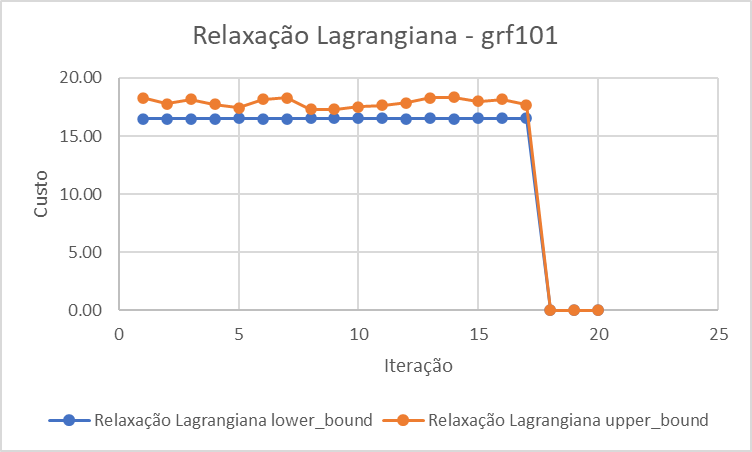
\includegraphics[width=\linewidth]{./images/grf101_RL.png}
        \caption{Relaxação Lagrangiana - grf101}
        \label{fig:grf101_RL}
    \end{minipage}
    \hfill
    \begin{minipage}{0.48\textwidth}
        \centering
        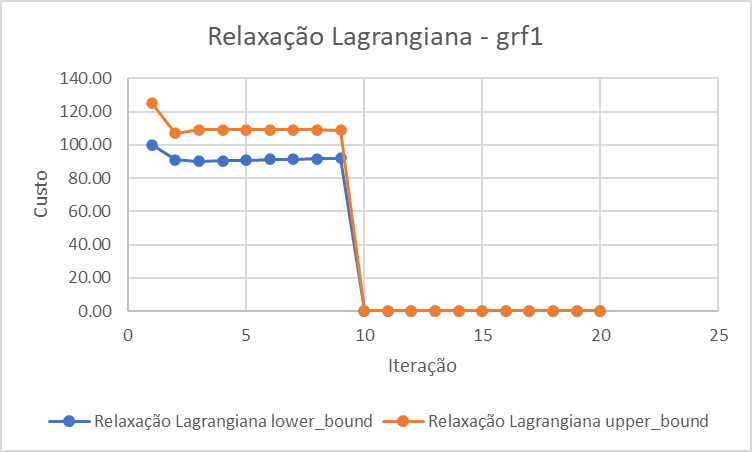
\includegraphics[width=\linewidth]{./images/grf1_RL.png}
        \caption{Simulated Annealing - grf101}
        \label{fig:grf101_SA}
    \end{minipage}
\end{figure}

Para o caso do \emph{Simulated Annealing} (\autoref{fig:grf101_SA} e \autoref{fig:grf1_SA}), notam-se picos na execução do algoritmo ao longo das iterações, o que é um comportamento esperado para essa metaheurística. A parametrização, apesar de básica, conseguiu gerar diversidade nas soluções e, de certa forma, explorar as possibilidades. No que diz respeito ao uso de tempo, para as instâncias pequenas, o tempo limite de $10$ minutos para cada uma foi suficiente para execução total de cada passo. Para \emph{grf101} a RL utilizou $515.0$ segundos e para o SA $339.0$ segundos. Já para a \emph{grf1}, a RL utilizou $279.0$ segundos (\emph{early stop} citado anteriormente) e para o SA $605.0$ segundos.

\begin{figure}[H]
    \centering
    \begin{minipage}{0.48\textwidth}
        \centering
        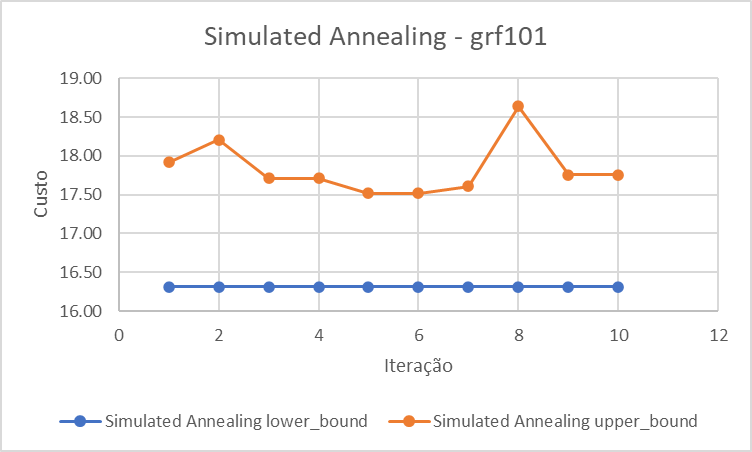
\includegraphics[width=\linewidth]{./images/grf101_SA.png}
        \caption{Relaxação Lagrangiana - grf1}
        \label{fig:grf1_RL}
    \end{minipage}
    \hfill
    \begin{minipage}{0.48\textwidth}
        \centering
        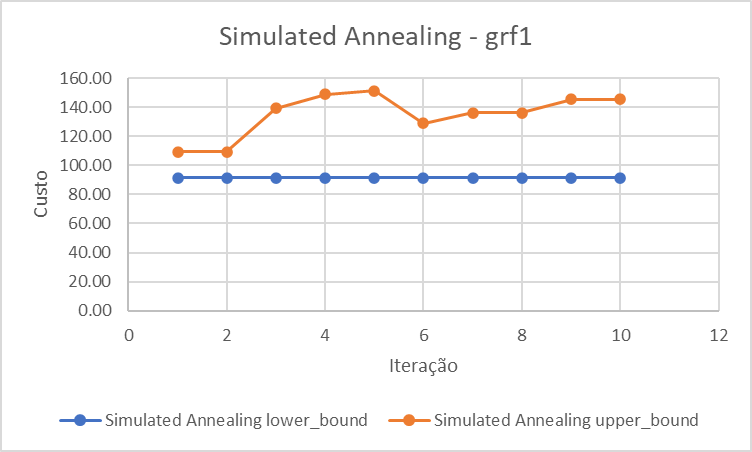
\includegraphics[width=\linewidth]{./images/grf1_SA.png}
        \caption{Simulated Annealing - grf1}
        \label{fig:grf1_SA}
    \end{minipage}
\end{figure}

Para as instâncias médias e grandes selecionadas, \emph{grf8, grf112, grf18 e grf129}, infelizmente, foram encontradas barreiras com relação ao uso de memória para a execução tanto da Relaxação Lagrangiana, pois o número de gatilhos estoura a memória para o vetor de violações, especialmente para a restrição $C10$; e também para o SA, pois o modelo continua grande demais para o tempo limite dividido entre as iterações, atingindo $60$ segundos ainda durante a fase de \emph{pre-solve} do Gurobi.

Porém, para o ILP foi possível construir os modelos inteiros e iniciar a otimização, como mostra a \autoref{tab:resultados-tatsp-ilp}. Apesar de não atingir \emph{gaps} razoáveis para os casos em questão, foi ao menos possível obter uma solução viável, exceto para a instância \emph{grf129}. E, Com exceção à instância \emph{grf101}, considerada a menor, todas as outras atingiram o tempo limite sem alcançar valores ótimos. Apesar disso, para as instâncias menores, foi possível notar que os limitantes alcançados são representativos para os valores encontrados pelo \emph{solver}, ou seja, limitam superior e inferiormente o ótimo do problema original.


\begin{table}[H]
\centering
\begin{tabular}{|c|c|c|}
\hline
\textbf{Instâncias} & \textbf{Custo} & \textbf{Status} \\
\hline
grf101 & 16.94   & OPTIMAL      \\
grf1   & 101.70  & TIME\_LIMIT   \\
grf112 & 50.93   & TIME\_LIMIT   \\
grf8   & 223.43  & TIME\_LIMIT   \\
grf129 & 0.00    & OUT\_OF\_MEMORY \\
grf18  & 355.55  & TIME\_LIMIT   \\
\hline
\end{tabular}
\caption{ILP para as seis instâncias.}
\label{tab:resultados-tatsp-ilp}
\end{table}

Por último, foi realizado um experimento focado na instância \emph{grf101} visando observar o desempenho da Relaxação Lagrangiana para diferentes dualizações das restrições de gatilhos. A \autoref{tab:dualizacao-limits} mostra como a dualização de restrições afeta os resultados mesmo em instâncias pequenas. A medida em que aumentamos o número de restrições dualizadas, nota-se uma piora na produção de limitantes, tanto inferiores quanto superiores. A queda mais brusca está ligada à restrição C10, tanto em tempo quanto qualidade. A suspeita mais forte é de que esse seja um conjunto de restrições muito grande, por ser construído aos pares de gatilhos, dois a dois. Além disso, isso afeta mais ainda a penalização da função objetivo.

\begin{table}[H]
\centering
\begin{tabular}{|c|c|c|c|c|c|c|c|}
\hline
\textbf{C6} & \textbf{C7} & \textbf{C8} & \textbf{C9} & \textbf{C10} & \textbf{Lower Bound} & \textbf{Upper Bound} & \textbf{Time(s)} \\
\hline
\checkmark & \ding{55} & \ding{55} & \ding{55} & \ding{55} & 16.53 & 17.32 & 515.0\\
\checkmark & \ding{55} & \ding{55} & \checkmark & \ding{55} & 16.51 & 17.32 & 606.0\\
\checkmark & \ding{55} & \ding{55} & \checkmark & \checkmark & 16.42 & 17.75 & 98.0\\
\checkmark & \checkmark & \checkmark & \checkmark & \checkmark & 16.30 & 17.57 & 5.0\\
\hline
\end{tabular}
\caption{Impacto da dualização progressiva das restrições C6-C10 sobre os limitantes inferior e superior.}
\label{tab:dualizacao-limits}
\end{table}

E, por último, vale citar que, ao dualizar restrições que contém \emph{Big M}, é notável a queda no tempo de execução, porém também nota-se uma flutuação expressivamente maior nos valores das violações, gerando problemas até de grandeza quando não controlados.